% ANEXO------------------------------------------------------------------------

\begin{anexosenv}
\partanexos

% Primeiro anexo---------------------------------------------------------------
\chapter{ESP-12S e ESP-12E}     % edite para alterar o título deste anexo
\label{chap:anexoA}

%Lembre-se que a diferença entre apêndice e anexo diz respeito à autoria do texto e/ou material ali colocado.

%Caso o material ou texto suplementar ou complementar seja de sua autoria, então ele deverá ser colocado como um apêndice. Porém, caso a autoria seja de terceiros, então o material ou texto deverá ser colocado como anexo.

%Caso seja conveniente, podem ser criados outros anexos para o seu trabalho acadêmico. Basta recortar e colar este trecho neste mesmo documento. Lembre-se de alterar o "label"{} do anexo.

%Organize seus anexos de modo a que, em cada um deles, haja um único tipo de conteúdo. Isso facilita a leitura e compreensão para o leitor do trabalho. É para ele que você escreve.

Este anexo abordará a respeito das características dos componentes ESP-12S e ESP-12E. Ambos possuem em seu interior o microcontrolador da Tensilica ESP8266EX. Esse microncontrolador pode ser programado por meio das linguagens C/C++, LUA e Micropython\cite{Embarcados}. o que tornam esses microntroladores interessantes são os recursos de Wi-Fi contidos. Ele integra interruptores de antena, \textit{balun} RF, amplificador de potência, filtros e módulos de gerenciamento de energia.

\section{Características gerais}

\begin{itemize}
	\item 11 GPIO's disponíveis para programação, possuindo barramentos 2C, SPI, UART, entrada ADC e saída PWM;
	\item Sensor interno de tempertura;
	\item CPU que opera em 80MHz, com possibilidade de operar em 160MHz (\textit{overclock});
	\item Arquitetura RISC 32 bits;
	\item 32KBytes de RAM para instruções;
	\item 96KBytes de RAM para dados;
	\item 64KBytes de ROM para boot;
	\item Memória Flash SPI Winbond W25Q40BVNIG de 512KBytes;
\end{itemize}

\begin{figure}[H]
	\centering
	\caption{Representação \textit{pinout} \textit{ESP-12E}}
	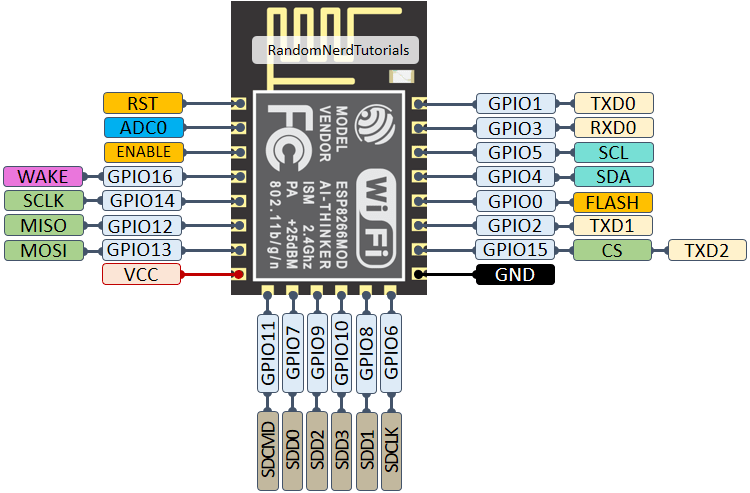
\includegraphics[width=0.9\textwidth]{figuras/ESP-12E_pinout.png}
	\fonte{Random Tutorials, 2019}
	\label{fig:esp12e_pinout}
\end{figure} 

\section {Caracteríticas Específicas}




\begin{table}[]
	\centering
	\small
	\newcolumntype{L}{>{\centering\arraybackslash}m{3cm}}
	\begin{tabular}{c|c|c|c}
		\hline
		\textbf{Pino} & \textbf{Direção} & \textbf{Descrição} & \textbf{Particularidade} \\ \hline
		
		GPIO 0 & INPUT / OUTPUT & \multicolumn{1}{m{6cm}|}{Usado para selecionar o modo de inicialização. Estando no \textit{GND} durante o \textit{boot}, entra no modo de \textit{flash}. Para inicialização normal manter contato com o \textit{VCC} ou deixá-lo em aberto.} & \multicolumn{1}{m{4cm}}{\textit{HIGH} na inicialização com oscilações por 120 \textit{ms}.} \\ \hline
		
		GPIO 1 & OUTPUT & \multicolumn{1}{m{6cm}|}{Usado como um UART0 TX durante a programação da \textit{flash}. Em modo de operação normal, pode ser utilizado como um GPIO de saída.} &  \multicolumn{1}{m{4cm}}{\textit{HIGH} na inicialização com oscilações por 80 \textit{ms}.} \\ \hline
		
		GPIO 2 & INPUT / OUTPUT & \multicolumn{1}{m{6cm}|}{De uso geral. Geralmente conectado à um \textit{LED}. Não permite o \textit{boot} se, na operação, for colocado em nível lógico baixo.} & \multicolumn{1}{m{4cm}}{\textit{HIGH} na inicialização com oscilações por 80 \textit{ms}.}\\ \hline
		
		GPIO 3 & INPUT & \multicolumn{1}{m{6cm}|}{Usado como um UART0 RX durante a programação da \textit{flash}. Em modo de operação normal, pode ser utilizado como um GPIO de saída.} & \multicolumn{1}{m{4cm}}{Permanace em nível lógico alto durante o \textit{boot}.}\\ \hline
		
		GPIO 4 & INPUT /OUTPUT & \multicolumn{1}{m{6cm}|}{Frequentemente usado como \textit{SCL} para \textit{I2C} (qualquer outro pino também pode ser usado). No modo de operação normal, ele pode ser usado como um GPIO clássico.} & \multicolumn{1}{m{4cm}}{Permanace em nível lógico baixo durante o \textit{boot}.}\\ \hline
		
		
		
		
	\end{tabular}
	\caption{}
	\label{tab:ta}
\end{table}
% https://www.tablesgenerator.com



% Novo anexo-------------------------------------------------------------------
\chapter{Raspberry Pi Zero W}
\label{chap:anexoB}

conteúdo do outro anexo

\end{anexosenv}
